\documentclass[english]{DESCARWINreport}

\usepackage{times}
\usepackage{helvet}
\usepackage{courier}
\usepackage{graphicx}
\usepackage{multirow}
%\usepackage[utf8]{inputenc}
\usepackage{algorithm}
\usepackage[noend]{algorithmic}
\usepackage{amsmath}
\usepackage{amsfonts}
\usepackage{amssymb}
\usepackage{array}
\usepackage{subfigure}
\usepackage{lscape}

\algsetup{indent=1.8em}
\renewcommand{\algorithmiccomment}[1]{// #1}
\newcommand{\pp}{planning tasks}
\newcommand{\PP}{planning task}
\newcommand{\dae}{{\em Divide-and-Evolve}}
\newcommand{\DAEI}{{\sc D\&E}}
\newcommand{\DAEII}{{\sc DaE2}}
\newcommand{\DAE}{{\sc DaE}}
\newcommand{\DAEX}{{\sc DaE$_{\text{X}}$}}
\newcommand{\DAEYAHSP}{{\sc DaE$_{\text{YAHSP}}$}}
\newcommand{\CPT}{{\sc CPT}}
\newcommand{\LPG}{{\sc LPG}}
\newcommand{\LAMA}{{\sc LAMA}}
\newcommand{\TFD}{{\sc TFD}}
\newcommand{\YAHSP}{{\sc YAHSP}}
\newcommand{\OPENSTACKS}{{\sc Openstacks}}
\newcommand{\ELEVATORS}{{\sc Elevators}}
\newcommand{\CREWPLANNING}{{\sc CrewPlanning}}
\newcommand{\FLOORTILE}{{\sc Floortile}}
\newcommand{\PARCPRINTER}{{\sc ParcPrinter}}

\def\MULTIZENO{{\sc MultiZenoTravel}}
\def\MONOZENO{{\sc ZenoTravel}}


\def\UU{{\mathbb{U}}}

%\title{DESCARWIN\\\bigskip {\em \LARGE The Marriage of Descartes and Darwin}\\\bigskip \bigskip \bigskip \bigskip \bigskip \bigskip \bigskip {\LARGE WP1: the \DAEX\ Planning System}}
\title{DESCARWIN\\\bigskip {\em \LARGE The Marriage of Descartes and Darwin}\\\vspace{8cm} {\LARGE D3.1: Design of a Benchmark Test Suite for Multi-Objective Evolutionary Planning}}
%ANR-09-COSI-002
%\author{Pierre Sav�ant}
\date{\today}
\laboratory{TRT - INRIA - ONERA}
\docref{62 441 217-179-1}

\revision{-}

\setlength{\parindent}{0cm}
\setlength{\parskip}{2ex plus 0.5ex minus 0.2ex}


% Pour r�duire globalement l'espace entre les items d'une liste
% on peut �galement utiliser le bout de code suivant de M. Wooding
% Les param�tres utilis�s pour d�finir cette mise en page
% sont les suivants :
% \topsep espace vertical suppl�mentaire (ajoute � \parskip)
%     ins�r� entre le texte pr�c�dant la liste et le 1er objet
%     de la liste
% \partosep espace vertical suppl�mentaire ins�r� devant la liste
%     si celle-ci est pr�c�d�e d'une ligne blanche
% \itemsep espace vertical suppl�mentaire (ajout� � \parsep)
%     ins�r� entre les �l�ments d'une liste.

%%%% debut macro %%%%
% \makeatletter
% \toks@\expandafter{\@listI}
% \edef\@listI{\the\toks@\setlength{\parsep}{0pt}}
% \edef\@listI{\the\toks@\setlength{\topsep}{0pt}}
% \makeatother
%%%% fin macro %%%%


\begin{document}

\maketitle

%\cleardoublepage

\begin{revisions}
\begin{revtable}
\dates{JUNE. 30, 2012}{}{}{}
\writers{Mostepha R. Khouadjia\\Marc Schoenauer\\Pierre Sav\'eant}{}{}{}
\approvers{P. Sav\'eant}{}{}{}
\end{revtable}
\begin{revisionlabels}
\revlabel{initial version}
\revlabel{}
\end{revisionlabels}
\end{revisions}

\begin{abstract}
This document provides the description of the multi-objective test suite that has been designed in the DESCARWIN project. Two goals were envisioned: on the one hand, because no such suite exists in the multi-objective context (whereas the successive International Planning Competitions (IPC) have lead to numerous recognized test suites for the single-objective case), it was necessary to have some problems on which to validate the multi-objective version of the  \DAEX\ planning system. On the other hand, we aim at starting for the multi-objective setting what has been achieved in the single-objective one, and established some recognized benchmarks in order to be able to compare different approaches to multi-objective planning. Ultimately, we would like to propose a new ``multi-objective track'' in the forthcoming IPCs, and stimulate research in that direction, as we are convinced that many real-world applications in fact require multi-objective techniques.

\end{abstract}

\tableofcontents

\newpage

\chapter{Introduction}
\section{Multi-objective planning}
Most real-world applications are multi-objective by nature. Typical situations in real-life involve some quality criterion associated with some cost -- and quality and cost are always contradictory objectives. In temporal planning for instance, the goal is to minimize the duration of a given plan: the quality is the makespan. But in real life, going fast has a cost, and very often it is possible to decrease the cost only at the expense of the duration. In such situations, the goal of optimization is not to find the best solution: only the decision-maker can decide what is best: going very fast at a very high cost, or going a little slower, but at a much lower cost. The name of the game then becomes {\em multi-objective optimization} and the goal is to provide the decision-maker with the best set of options from which to choose from, what is called Pareto-optimal solutions, i.e. such solutions that no other solution is better on all objectives.

However, very little attention has been paid in the AI Planning community to multi-objective  -- despite the fact that most real-life planning problems are, like other real problems, multi-objective by nature. One reason for that proably comes from the history of planners, that have been derived from AI methods like constraint programming, graph theory, and the like - domains where a single objective is mandatory. As a consequence, even though multi-objective planning problems begin to raise some interest, there exist to-date no benchmark of multi-objective AI planning problems. This is in high constrast with the single-objective case: due to the very high success of the International Planning Competitions (IPC) over the years, a very large body of benchmark problems has been validated and adopted by the whole AI Planning community.

One of the goals of the DESCARWIN project is to provide the first bricks of a similar testbed for multi-objective planning optimization -- and this deliverable is a first step in that direction.

\section{Survey of proposed approaches}
Two different approaches have been used to design a first benchmark suite for multi-objective AI planning. Firstly, starting from a very simple toy problem inspired by the {\tt zeno} logisitic domain of all IPCs (probably the most widely used domain, including 30 instances of increasing difficulty), a series of problems have been design, with parameterized complexity, and for which the exact Pareto front can be easily exactly known (at least for the simplest instances). Because the domain pertains to logistic, the first (main?) objective remains the total duration of the resulting plan. A second objective has been introduced, and two different types of objectives have been proposed: a ``cost'', for which every segment of transportation has a given cost, and the total cost is the sum of all costs, and a ``risk'' for which every segment has a given risk, and the total risk is the maximum encountered risk during the execution of the plan.

Secondly, the huge reservoir of domains that have been carefully tuned over the years by the IPC competitions contains many good candidate domains for ``multi-objectivization``, and based on the semantics of those domains, we have proposed ad hoc extensions of these domains to multi-objective setting.


\chapter{Zeno-based 'toy' problems}
\section{The (single-objective) zeno domain}
This Section describes the simple problems derived from the {\tt zeno} single-objective domain, probably the most well-know domain of AI planning after the STRIP block world, that has been present in all IPC competitions since the beginning. 

The {\tt zeno} domain involves persons, cities and planes. States describe in which city each person and each plane is located (predicate {\tt at} with two arguments, a city and a person or a plane), and the fuel-level of each plane. Actions allow persons to bord/unboard a plane, planes to travel from one city to another (with whoever is on-board), either fast (and consuming a lot of fuel) or slowly (with low fuel consumption), and planes to refuel. All actions have a duration. See Annex \ref{zenoMultiDomain} for the domain file.

We will use here a simplified {\tt zeno} domain, where there is no fuel level, no boarding/unboarding actions. This simple domain (for single objective optimization) is written in PPDL as follows. There are only 2 actions, {\tt fly} and {\tt flyVide} that move the planes with or without a passenger, and the preconditions and effects of the actions are rather straightforward.

\begin{verbatim}
(:action fly
 :parameters (?a ?c1 ?c2 ?x)
 :duration (= ?duration (timeTravel ?c1 ?c2))
 :precondition
    (and (aircraft ?a) (city ?c1) (city ?c2)    
             (at ?a ?c1) (person ?x) (at ?x ?c1) 
        )
 :effect
    (and (at ?a ?c2) (not (at ?a ?c1)) 
             (not (at ?x ?c1)) (at ?x ?c2)
        )
)

(:action flyVide
 :parameters (?a ?c1 ?c2)
 :duration (= ?duration (timeTravel ?c1 ?c2))
 :precondition
    (and (aircraft ?a) (city ?c1) (city ?c2) (at ?a ?c1) 
        )
 :effect
    (and (at ?a ?c2) (not (at ?a ?c1))
        )
)
\end{verbatim}


A given instance must instantiate all variables. The simplest non-trivial instance is symbolically represented on Figure \ref{fig:monoZeno}: it has 3 cities, and 3 persons must be transported from city0 to city2 using 2 planes that are in city0 in the initial state as well. Flights only exist from city0 to city1 and city1 to city2, and have the same duration of 2, not depending on whether the plane is full or empty. The advised reader will rapidly find the non-trivial solution with a total makespan of \ldots 8!


\begin{figure}[tb!]
  \begin{center}
 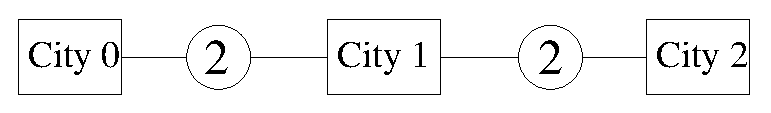
\includegraphics[width=0.5\textwidth]{miniMono.eps}
 % instance.eps: 0x0 pixel, 300dpi, 0.00x0.00 cm, bb=0 0 509 388
\caption{A schematic view of the simple \MONOZENO\ instance used as a basis for the MultiZeno design: the domain is a simplified version of the standard {\tt zeno} domain regarding transportation problems: There are only 3 cities, and 2 possible flights whose durations are attached to the corresponding edges.}
\label{fig:monoZeno}
\end{center}
\end{figure}

This problem corresponds to the PDDL file containing as initial and final goal the following lines, that are self-explaining.
\begin{verbatim}
(:init
    (= (timeTravel city0 city1) 2)
    (= (timeTravel city1 city0) 2)

    (= (timeTravel city1 city2) 2)
    (= (timeTravel city2 city1) 2)

    (at plane1 city0)
    (at plane2 city0)
    (at person1 city0)
    (at person2 city0)
    (at person3 city0)
)
(:goal (and
    (at person1 city2)
    (at person2 city2)
    (at person3 city2)
    )
)
\end{verbatim}
Note that the initial goal contains the definitions of the duration (through ''function`` {\tt timeTravel}), as well as the localization of {\bf all} objects (2 planes and 3 persons) while the goal state only contains a partial description of a state (all persons in city2). The instance PDDL file also contains the definitions and types of all objects, referring to the domain PDDL file (see in Appendix at end of this deliverable).


\section{The multi-objective zeno domain}
\label{sec:simpleZenoMulti}
\begin{figure}[tb!]
  \begin{center}
 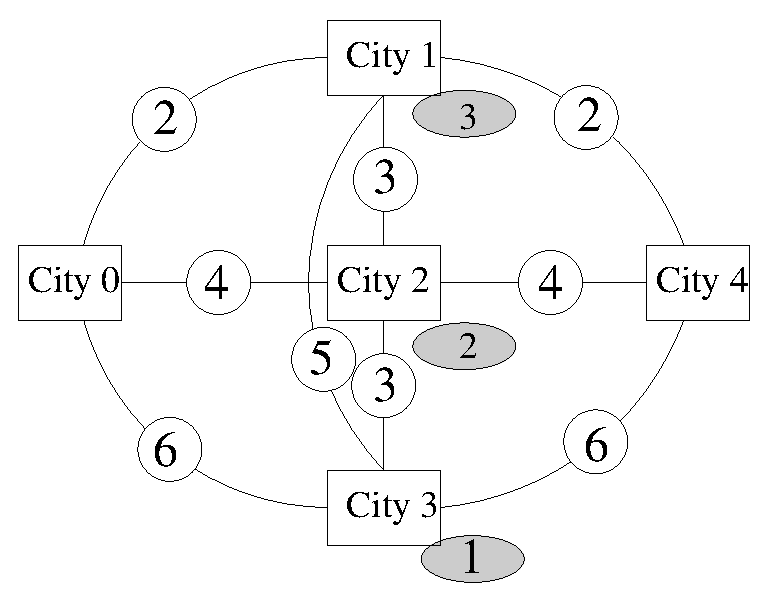
\includegraphics[width=0.5\textwidth]{miniMulti.eps}
 % instance.eps: 0x0 pixel, 300dpi, 0.00x0.00 cm, bb=0 0 509 388
\caption{A schematic view of a \MULTIZENO\ instance, the proposed simple benchmark transportation problem: Durations of available flights are attached to the corresponding edges, costs/risks are attached to landing in the central cities (in gray circles).}
\label{fig:multiZeno}
\end{center}
\end{figure}


This section will detail the simple domain for multi-objective temporal planning that is described in Figure \ref{fig.instance}. The reader will have by now solved the little puzzle set in previous Section, and found the solution with makespan 8 (flying 2 passengers to {\tt city1}, one plane continues with its passenger to {\tt city2} while the other plane flies back empty to {\tt city0}, the plane in {\tt city2} returns empty to {\tt city1} while the other plane brings the last passenger there, and the goal is reached after both planes bring the two remaining passengers to {\tt city2}). 

\subsection{The simple multi-objective zenoTravel3 problem}
In order to turn this problem into a not-too-unrealistic multi-objective problem, there are now 3 possible intermediate cities, with different travel time to the two outer cities (0 and 4 in the example of Figure \ref{fig:multiZeno}), and another objective is added, that is increased when landing on any of the 3 central cities (cities 1 to 3 in the same example). In order to make the objective contradictory, this second objective varies inversely to the first one, being large for city1 that is fast to reach, and small for city3 to where travel takes more time. There are however (at least) two ways to take this objective into account during a complete plan, that lead to two types of problems: In the \MULTIZENO$_{Cost}$, the second objective is similar to a cost, i.e. is increased additively: each plane has to pay the corresponding tax every time it lands one of the taxed cities; In the \MULTIZENO$_{Risk}$, the second objective is similar to a risk, and the maximal value encountered during the complete execution of a plan is to be minimized. 

In both cases however, there are 3 obvious points that belong to the Pareto Front: the solution with minimal makespan described in the single-objective case, going from city0 to city4 through city1, and the similar solutions that use respectively {\tt city2} and {\tt city3} in lieu of {\tt city1}. The values of the makespans are respectively 8, 16 and 24, and the values of the costs are, for each solution, 4 times the value of the single landing tax, and exactly the highest value in case of risk. For the risk case, there is no other point on the Pareto Front, as a single landing on a high-risk city sets the risk of the whole plan to that high risk. For the cost problem, however, there are other points on the Pareto Front, as different cities can be used for the different passengers. For instance, in the case of Figure \ref{fig:multiZeno}, this leads to a Pareto Front made of 5 points, (8,12), (16,8), and (24,4) (going only through {\tt city 1}, {\tt 2} and {\tt 3} respectively), plus (12,10) and (20,6). It should be noted that these two Pareto-optimal solutions, like the 3 first 'elementary' solutions already mentionned, also use some tricky way to use all available resources: 

\subsection{Multi-objective PDDL files}
The PDDL files are modified to take into account the second objective. Fortunately, within PDDL 2.0, there already exists a mechanism to handle ''actions with cost`` - one of the recognized types of AI planning problems, in which each action has a cost, and the total cost is to be minimized. This mechanism was used here, hence avoiding the need to redefine any part of the PDDL language.

In the domain file, one needs to first indicate in the header that actions will have a cost, with the line
\begin{verbatim}
  (:requirements :strips :durative-actions :action-costs)
\end{verbatim}
Another line is used to indicate how this cost will be computed, using functions {\tt total-cost} to carry the cost along a plan, and function {\tt cityThreat} to compute the local 'cost' or 'risk'. This is done by adding these 2 functions to the function declaration
\begin{verbatim}
  (:functions (citythreat ?x) (timeTerre ?x ?y) (total-cost)
\end{verbatim}

Finally, the effects of the {\tt fly} and {\tt flyVide} actions must include some update of the {\tt total-cost}, with the line
\begin{verbatim}
    (increase (total-cost) (citythreat ?c2)) 
\end{verbatim}


In the instance file, the initial state must initialize the {\tt total-cost}, and define, for each city, the second objectives {\tt cityThreat}. This is done with the following lines, that are included inside the {\tt init} state.
\begin{verbatim}
    (= (total-cost) 0)
    (= (citythreat city0) 0)
    (= (citythreat city1) 100)
    (= (citythreat city2) 10)
    (= (citythreat city3) 1)
    (= (citythreat city4) 0)
\end{verbatim}

The complete resulting files for zeno3 (i.e. the simplest instance with 3 persons) can be seen in the Annex, and the corresponding two Pareto fronts are represented on Figure \ref{fig:zeno3Fronts}.

\subsection{Cost or Risk?}
\label{costOrRisk}
Whether the secondary objective should be considered additive (partial costs are added over the complete plan) or ''maxitive`` (the risk of a plan is the maximum of all risk values encountered when executing an action of the plan) could not have been introduced in PPDL without extending the existing language - and adding new features unilaterally has the poor consequence that your PPDL files are not compatible with other people solvers any more. Hence we have chosen to let the embedded solver handle this: at the moment, the API for YASHP includes a switch between additive and maxitive total-cost.

It is also important to note that even though DaE is now multi-objective, the embedded solver remains single-objective, and is not aware that the problem is multi-objective. It can only be told that the objective (to minimize) is the makespan (or the total cost), and to simply propagate the other objective in the end -- which is what is done anyway to compute the overall makespan or cost. So here again, no overhead on the solver's side.
But this will of course be much more detailed in the next deliverable, together with the results obtained by DaE.


\section{A sequence of multi-objective zeno-based instances}

\subsection{Increasing the Complexity}
There are several ways to make this first simple instance more or less complex. A first possibility is to modify the relative values of the taxes/risks on the central cities: for instance, the two sets of values that have been experimented with in the first experiments with this benchmark are the (3-2-1) case depicted on Figure \ref{fig:multiZeno}, and the (100-10-1) case, somehow representing another extreme of the spectrum of possible values.

A second way is to add passengers. Sticking to bunches of 3 passengers in order to be able to easily derive some obvious Pareto-optimal solutions, it is easy to derive all the solutions for 6 and 9 passengers (see the corresponding Pareto fronts on Figure \ref{fig:zeno6} and \ref{fig:zeno9}).

Finally, the number of central cities can also be increased: this creates more points on the Pareto front, be they plans in which a single city is used for all passengers or plans that use several different cities for different passengers (still using the same trick to ensure no plane ever stays idle).

Of course, the number of planes could also be increased, but the number of passengers would need to remain larger than the number of planes, and the Pareto front would not stay as easily identifiable than with 2 planes.

\subsection{Modifying the shape of the Pareto Front}

Another way to modify the difficulty of the problem without increasing its complexity is to tune the different values of the flight times and the cost/risk at each city. such changes will not modify the number of points on the Pareto Front, but will certainly change its shape in the objective space. For instance, simply modifying the cost $\alpha$ of {\tt city2}, the central city in Figure \ref{fig:multiZeno}, between 1 and 3 (the costs of respectively {\tt city1} and {\tt city3}), the Pareto Front, which is linear for $\alpha=2$ becomes strictly convex for $\alpha < 2$ and strictly concave for $\alpha > 2$, as can be seen on Figure \ref{fig:ParetoFronts}.


\chapter{Multi-Objectivization of IPC domains}
%%%%%%%%%%%%%%%%%%%%%%%%%%%%
\label{testbench}
This section presents the family of benchmark problems that have derived from the IPC single-objective domains. 

% MINI ZENO

\section{IPC-7 Domains}
Two satisficing tracks were open at IPC-7: sequential satisficing, i.e., sequential STRIPS planning in which actions have a cost and the total cost is to me minimized, and temporal satisficing, where actions have a duration and can be run in parallel if all resources are available at the same time -- and the total makespan is to be minimized. 
Some domains appeared in both tracks, with the same instances (i.e. instances with the same objects), and from these domains, we could generate problems with 2 objectives, the duration (makespan) and the cost (or risk, as in Section \ref{costOrRisk}). Note that domains where action durations or costs were uniformly equal to one were rejected outright.

The domain PPDL files were generated by hand, while the PDDF for the instances were automatically generated by some Python script from both corresponding instances of tht two domains (sequential with costs and temporal).

Five domains were handled that way: \ELEVATORS, \CREWPLANNING, \FLOORTILE, \OPENSTACKS, and \PARCPRINTER.
They are detailed in turn in the following Sections, as the way the actual multi-objectivization is done slightly varies from one domain to another, despite the fact that all had sequential and temporal instances.


Indeed, though the underlying rationale for multi-objectivization is always something around ''withmore resource,  things get done faster, but cost more``, it turned out that in order to get non-trivial Pareto fronts, some modifications to the ''direct-product`` of the sequential and the temporal domains had to be done.

Note also that more domains could be ''multi-objectivized'' using similar techniques, even those without that do not already have sequential and temporal instances. 


\section{\ELEVATORS}

\subsection{The domain}
%The \ELEVATORS\ domain is stated as follows: there is a building with $N+1$ floors,
%numbered from $0$ to $N$. The building can be separated in blocks of size $M+1$, where
%$M$ divides $N$. Adjacent blocks have a common floor. The building has $K$ fast
%(accelerating) elevators that stop only in floors that are multiple of $M/2$. 
%Each fast elevator has a capacity of $X$ persons.
%Furthermore, within each block, there are $L$ slow elevators, that stop at every
%floor of the block. Each slow elevator has a capacity of $Y$ persons (usually
%$Y<X$). There are costs associated with each elevator starting/stopping and
%moving. There are several passengers, for which their current location and their
%destination are given. The objective function is to minimize the total cost of
%moving the passengers to their destinations. The total cost is increased each
%time an elevator starts/stops or moves.


The idea for this domain came up from the Miconic domain of IPC2, however the domain has been designed from scratch. The scenario is the following: There is a building with N+1 floors, numbered from 0 to N. The building can be separated in blocks of size M+1, where M divides N. Adjacent blocks have a common floor. For example, suppose N=12 and M=4, then we have 13 floors in total (ranging from 0 to 12), which form 3 blocks of 5 floors each, being 0 to 4, 4 to 8 and 8 to 12.

The building has K fast (accelerating) elevators that stop only in floors that are multiple of M/2 (so M has to be an even number). Each fast elevator has a capacity of X persons. Furthermore, within each block, there are L slow elevators, that stop at every floor of the block. Each slow elevator has a capacity of Y persons (usually Y<X).

There are costs associated with each elevator starting/stopping and moving. In particular, fast (accelerating) elevators have negligible cost of starting/stopping but have significant cost while moving. On the other hand, slow (constant speed) elevators have significant cost when starting/stopping and negligible cost while moving.

Traveling times between floors are given for any type of elevator, taking into account the constant speed of the slow elevators and the constant acceleration of the fast elevators.

There are several passengers, for which their current location (i.e. the floor they are) and their destination are given. The planning problem is to find a plan that moves the passengers to their destinations while it maximizes some criterion.

In the sequential tracks the objective function is to minimize the total cost of moving the passengers to their destinations. The total cost is increased each time an elevator starts/stops or moves.

For the satisficing track, in the 2008 competition, problems ranged from 9 floors, 4 passengers, and 4 elevators (2 fast, 2 slow) to 25 floors, 39 passengers, and 5 elevators (2 fast, 3 slow). Initial capacity of fast elevators is 3 and of slow ones is 2. The 10 first problems of IPC 2008 increased the number of passengers by one from the previous problem. The number 11, doubled the floors and made passenger = 8, while increasing in one the elevators' capacity. From it, 2 passengers were added till problem 20. From problem 21, a slow elevator was added, the capacity was increased to 6 for fast lifts and to 4 for slow ones, the number of floors was raised to 25 and the number of passengers was 12 an was increased by 3 in each problem. During IPC 2008, competitor planners either only solved the 4-5 first problems or did not have trouble until the last ten.

For IPC 2011 the last 9 problems were reused, plus problem 14 (only solved by one planner like a bunch of other ones). The remaining 10 problems start from characteristics of old problem 30 (current problem 10), adding 2 fast elevators, 1 slow and 1 passenger. The next 4 increase the number of passengers by 3. From problem 16 floors are 40, 4 fast lifts with capacity for 6 passengers, 4 slow ones for 4 passengers, and 40 passengers, increasing the number of passengers in 5 per problem. 

\subsection{The multi-objectivization}
For \ELEVATORS\ a simple mixing of both sequential and temporal domains is straightforward: fast moves are more costly than slow moves. Hence the original values of the both objectives could be used as is, by simply adding the increasing/decreasing effect of the cost on the actions of the temporal domain. A typical action then looks like:

\begin{verbatim}
(:action move-up-slow
   :parameters (?lift - slow-elevator ?f1 - count ?f2 - count)
   :duration (= ?duration (travel-slow-temp ?f1 ?f2))
   :precondition (and (lift-at ?lift ?f1) 
                      (above ?f1 ?f2 )
                      (reachable-floor ?lift ?f2) )
   :effect (and (lift-at ?lift ?f2) 
                (not (lift-at ?lift ?f1)) 
                (increase (total-cost) (travel-slow-cost ?f1 ?f2))))
\end{verbatim}
See details in the complete listings in the Annex.

\section{\CREWPLANNING, \FLOORTILE, and \PARCPRINTER}

\subsection{Multi-objectivization}
For \CREWPLANNING, \FLOORTILE, and \PARCPRINTER, the existing values of the cost did not ensure that both objectives would be in conflict. Hence, it was decided to arbitrarily set the cost values to the inverse of the duration, thus ensuring the antagonism of both objectives. A typical action from the \CREWPLANNING\ domain then looks like:

\begin{verbatim}
(:durative-action change_filter
  :parameters (?fs - FilterState ?c - CrewMember ?d - Day)
  :duration (= ?duration 60)
  :condition (and (at start (available ?c))
                  (over all (currentday ?c ?d)))
  :effect (and (at start (not (available ?c)))
               (at end (available ?c))
               (at end (changed ?fs ?d))
               (increase (total-cost) (/ 1 60))))
\end{verbatim}


\subsection{\FLOORTILE\ domain}
A set of robots use different colors to paint patterns in floor tiles. The robots can move around the floor tiles in four directions (up, down, left and right). Robots paint with one color at a time, but can change their spray guns to any available color. However, robots can only paint the tile that is in front (up) and behind (down) them, and once a tile has been painted no robot can stand on it.

For the IPC set, robots need to paint a grid with black and white, where the cell color is alternated always. This particular configuration makes the domain hard because robots should only paint tiles in front of them, since painting tiles behind make the search to reach a dead-end.

\subsection{\PARCPRINTER\ domain}
This domain models the operation of the multi-engine printer, for which one prototype is developed at the Palo Alto Research Center (PARC). This type of printer can handle multiple print jobs simultaneously. Multiple sheets, belonging to the same job or different jobs, can be printed simultaneously using multiple Image Marking Engines (IME). Each IME can either be color, which can print both color and black\&white images, or mono, which can only print black\&white image. Each sheet needs to go through multiple printer components such as feeder, transporter, IME, inverter, finisher and need to arrive at the finisher in order. Thus, sheet (n+1) needs to be stacked in the same finisher with sheet n of the same job, but needs to arrive at the finisher right after sheet n (no other sheet stacked in between those two consecutive sheets). Given that the IMEs are heterogeneous (mixture of color and mono) and can run at different speeds, optimizing the operation of this printer for a mixture of print jobs, each of them is an arbitrary mixture of color/b\&w pages that are either simplex (one-sided print) or duplex (two-sided print) is a hard problem. For the detail description of this domain and the continual online planner controlling it, please refer to the references listed at the end of this page.

This domain is used in two tracks: sequential and temporal. The temporal track is the most natural fit due to the default objective function for the printer of maximizing its productivity, which equals to finish printing all print job requests as quickly as possible. For the sequential track, we use a more seldom used objective function of minimizing printing cost. For example, using a more expensive color IME to print a black\&white page costs more than using a mono IME. However, the cost tradeoff may not be clearcut if the feeder, where the blank sheets originally reside at is closer to the mono IME than to the color IME.

Overall, three different printers have been modeled, two with 2 IMEs (one color and one mono) and one with 4 IMEs (two colors and two monos). Two with rather symmetric design and a third one is asymmetric. Even those the printers are hypothetical, the hardware that can be used to make those printers are real.

For the problem files, to reduce complexity, print request of a single job with multiple sheets have been created. The sheets are randomly set to be either simplex (one-sided print) or duplex (two-sided print) and each image is also randomly selected to be either mono or color. The number of sheets varies from 1 to 20. Given this print job request and a particular printer configuration, the competing planner needs to find a plan with lowest total printing cost in the sequential track (matching well between image requirement and IME capabilities) and smallest makespan in the temporal track (synchronize well different IMEs).

There is no generator for this domain, so new problems will be by-hand generated using IPC 2008 ones. New problems will add some sheets to old problems or will make two-sided some of them. As in the IPC 2008, three different printers are used, one for problems 1-10, another for 11-20, and another for 21-30.

Remark: Printer 1 is not able to turn a page once printed, so if a problem prints something in the back side, the sheet needs to finish with back side up.

For the satisficing track, in the IPC 2008 the first problem had 1 sheet, second one 2 sheets and so on until problem 10. The same applies for problems 11-20 (changing the printer) and 21-30.

\section{\OPENSTACKS}
\subsection{The domain}

The \OPENSTACKS\ domain is based on the ``minimum maximum simultaneous open stacks''
combinatorial optimization problem, which can be stated as follows: a
manufacturer has a number of orders, each for a combination of different
products, and can only make one product at a time. The problem is to order the
making of the different products so that the maximum number of stacks that are
in use simultaneously, or equivalently the number of orders that are in
simultaneous production, is minimized. The problem is NP-hard and known to be
equivalent to several other problems. In the temporal case a maximum number of
stacks is given and the goal is to find the plan with the minimum makespan,
without violating the maximum number of stacks constraints.

\subsection{Muti-objectivization}
For \OPENSTACKS, the temporal version starts from a stack with a fixed size and tries to find the shortest trip whereas the cost version does not limit the size of the stack but adds an action of cost 1 for each stack opening. This action was simply added to the temporal version:

\begin{verbatim}
(:action open-new-stack
  :duration (= ?duration 1)
  :parameters (?open ?new-open - count)
  :precondition (and (stacks-avail ?open)
                     (next-count ?open ?new-open))
  :effect (and (not (stacks-avail ?open))
               (stacks-avail ?new-open) 
               (increase (total-cost) 1)))
\end{verbatim}


Syntaxically the two objectives are declared in the domain within the requirements slot:
\begin{verbatim}
(:requirements :typing :durative-actions :action-costs)
\end{verbatim}

The bi-objective metrics is specified in the problem with the following syntax:
\begin{verbatim}
(:metric (and (minimize (total-time)) (minimize (total-cost))))
\end{verbatim}


\chapter{Conclusion}
\label{conclusion}
This deliverable has introduced the benchmark test suite that has been designed for multi-objective AI planning. To the best of our knowledge, no such benchmark existed yet, as very little attention has been paid to multi-objective problems in AI planning until now. 

The proposed suite contains two types of problems.
First, for a simplified logistics domain inspired by the single-objective {\tt zeno} domain (i.e., transporting passengers between cities with limited number of planes), a set of 'toy' problems of parameterized complexity has been defined. They are toy problems because the exact Pareto front, or large parts of the exact Pareto fronts, can be theoretically identified (even if this becomes tedious as the complexity increases). But they can be made arbitrarily difficult by increasing the number of cities and/or the number of passengers, and tuning the values of the partial objective values.

The second set of problems comes from IPC-7 (single-objective) domains. For several of them, two series of almost identical instances existed, one in the temporal track, and one in the 'action-with-costs' track. Whenever possible, these were merged into multi-objective instances. For some other domaines, a secondary objective was arbitrarily set to a decreasing function of the makespan for each action, ensuring contradictory objectives. 

In both cases, XXXX





% \chapter{References}
% \bibliographystyle{plain}
% \bibliography{icaps10}
\begin{tiny}

\Roman{section}    
\setcounter{chapter}{6}
\chapter*{Annexes: PDDL files}
\section{\MULTIZENO\ PDDL domain file}
\label{zenoMultiDomain}
\begin{verbatim}(define (domain zeno-travel)
(:requirements :strips :durative-actions :action-costs)
(:predicates
     (at ?x ?c) (aircraft ?p) (person ?x) (city ?x) (libre ?x)
)
(:functions (citythreat ?x) (timeTerre ?x ?y) (total-cost)
)
(:action fly
 :parameters (?a ?c1 ?c2 ?x)
 :duration (= ?duration (timeTerre ?c1 ?c2))
 :precondition
    (and (aircraft ?a) (city ?c1) (city ?c2)    
             (at ?a ?c1) 
             (person ?x) (at ?x ?c1) (libre ?a)
        )
 :effect
    (and (at ?a ?c2) (not (at ?a ?c1)) 
             (not (libre ?a)) (libre ?a) (not (at ?x ?c1)) (at ?x ?c2)
         (increase (total-cost) (citythreat ?c2))
        )
)
(:action flyVide
 :parameters (?a ?c1 ?c2)
 :duration (= ?duration (timeTerre ?c1 ?c2))
 :precondition
    (and (aircraft ?a) (city ?c1) (city ?c2) (at ?a ?c1) 
        (libre ?a)
        )
 :effect
    (and (at ?a ?c2) (not (at ?a ?c1))
             (not (libre ?a)) (libre ?a)
         (increase (total-cost) (citythreat ?c2))
        )
)
)
\end{verbatim}

\section{A simple \MULTIZENO\ PDDL instance file}
\label{zeno3-123-instance}
This instance is a very simple exemple of a \MULTIZENO\ instance, with 3 passengers, 3 intermediate sities, 2 planes, and a linear Pareto Front (see Section \ref{sec:simpleZenoMulti}).
\begin{verbatim}
(define (problem ZTRAVEL-3-8)
(:domain zeno-travel)
(:objects
    plane1
    plane2
    person1
    person2
    person3
    city0
    city1
    city2
    city3
    city4
    )
(:init
    (= (total-cost) 0)
    (= (citythreat city0) 0)
    (= (citythreat city1) 100)
    (= (citythreat city2) 10)
    (= (citythreat city3) 1)
    (= (citythreat city4) 0)

        (= (timeTerre city0 city1) 2)
        (= (timeTerre city0 city2) 4)
        (= (timeTerre city0 city3) 6)
        (= (timeTerre city1 city4) 2)
        (= (timeTerre city2 city4) 4)
        (= (timeTerre city3 city4) 6)

        (= (timeTerre city1 city0) 2)
        (= (timeTerre city2 city0) 4)
        (= (timeTerre city3 city0) 6)
        (= (timeTerre city4 city1) 2)
        (= (timeTerre city4 city2) 4)
        (= (timeTerre city4 city3) 6)

        (= (timeTerre city1 city2) 3)
        (= (timeTerre city1 city3) 5)
        (= (timeTerre city2 city3) 3)

        (= (timeTerre city2 city1) 3)
        (= (timeTerre city3 city1) 5)
        (= (timeTerre city3 city2) 3)

    (at plane1 city0)
    (aircraft plane1)
    (at plane2 city0)
    (aircraft plane2)
    (at person1 city0)
    (person person1)
    (at person2 city0)
    (person person2)
    (at person3 city0)
    (person person3)
    (city city0)
    (city city1)
    (city city2)
    (city city3)
    (city city4)
        (libre plane1)
        (libre plane2)
)
(:goal (and
    (at person1 city4)
    (at person2 city4)
    (at person3 city4)
    ))
)
\end{verbatim}

\section{\ELEVATORS\ PDDL domain file}
\begin{verbatim}
; S�mantique temporelle conservative : on omet les modalit�s temporelles du bench original (YAHSP ne les traite pas)

(define (domain elevators-tempo-cost)
  (:requirements :typing :action-costs :durative-actions)
  (:types     elevator - object 
            slow-elevator fast-elevator - elevator
               passenger - object
              count - object
         )

(:predicates 
    (passenger-at ?person - passenger ?floor - count)
    (boarded ?person - passenger ?lift - elevator)
    (lift-at ?lift - elevator ?floor - count)
    (reachable-floor ?lift - elevator ?floor - count)
    (above ?floor1 - count ?floor2 - count)
    (passengers ?lift - elevator ?n - count)
    (can-hold ?lift - elevator ?n - count)
    (next ?n1 - count ?n2 - count)
)

(:functions (total-cost) - number
            (travel-slow-cost ?f1 - count ?f2 - count) - number
            (travel-fast-cost ?f1 - count ?f2 - count) - number 
            (travel-slow-temp ?f1 - count ?f2 - count) - number
            (travel-fast-temp ?f1 - count ?f2 - count) - number 
)

(:action move-up-slow
  :parameters (?lift - slow-elevator ?f1 - count ?f2 - count )
  :duration (= ?duration (travel-slow-temp ?f1 ?f2))
  :precondition (and (lift-at ?lift ?f1) (above ?f1 ?f2 ) (reachable-floor ?lift ?f2) )
  :effect (and (lift-at ?lift ?f2) (not (lift-at ?lift ?f1)) (increase (total-cost) (travel-slow-cost ?f1 ?f2))))

(:action move-down-slow
  :parameters (?lift - slow-elevator ?f1 - count ?f2 - count )
  :duration (= ?duration (travel-slow-temp ?f2 ?f1))
  :precondition (and (lift-at ?lift ?f1) (above ?f2 ?f1 ) (reachable-floor ?lift ?f2) )
  :effect (and (lift-at ?lift ?f2) (not (lift-at ?lift ?f1)) (increase (total-cost) (travel-slow-cost ?f2 ?f1))))

(:action move-up-fast
  :parameters (?lift - fast-elevator ?f1 - count ?f2 - count )
  :duration (= ?duration (travel-fast-temp ?f1 ?f2))
  :precondition (and (lift-at ?lift ?f1) (above ?f1 ?f2 ) (reachable-floor ?lift ?f2) )
  :effect (and (lift-at ?lift ?f2) (not (lift-at ?lift ?f1)) (increase (total-cost) (travel-fast-cost ?f1 ?f2))))

(:action move-down-fast
  :parameters (?lift - fast-elevator ?f1 - count ?f2 - count )
  :duration (= ?duration (travel-fast-temp ?f2 ?f1))
  :precondition (and (lift-at ?lift ?f1) (above ?f2 ?f1 ) (reachable-floor ?lift ?f2) )
  :effect (and (lift-at ?lift ?f2) (not (lift-at ?lift ?f1)) (increase (total-cost) (travel-fast-cost ?f2 ?f1))))

(:action board
  :parameters (?p - passenger ?lift - elevator ?f - count ?n1 - count ?n2 - count)
  :duration (= ?duration 1)
  :precondition (and  (lift-at ?lift ?f) (passenger-at ?p ?f) (passengers ?lift ?n1) (next ?n1 ?n2) (can-hold ?lift ?n2) )
  :effect (and (not (passenger-at ?p ?f)) (boarded ?p ?lift) (not (passengers ?lift ?n1)) (passengers ?lift ?n2) ))

(:action leave 
  :parameters (?p - passenger ?lift - elevator ?f - count ?n1 - count ?n2 - count)
  :duration (= ?duration 1)
  :precondition (and  (lift-at ?lift ?f) (boarded ?p ?lift) (passengers ?lift ?n1) (next ?n2 ?n1) )
  :effect (and (passenger-at ?p ?f) (not (boarded ?p ?lift)) (not (passengers ?lift ?n1)) (passengers ?lift ?n2) ))
  
) 
\end{verbatim}

\section{\ELEVATORS\ PDDL instance file {\tt p01-p04-temp-cost.pddl}}
% This is one of the simplest instances of the \ELEVATORS\ domain -- 2 fast and 2 slow elevators, for 25 passengers and 16 floors.
\begin{tt}
(define (problem elevators-time-cost-p01-p04)
(:domain elevators-tempo-cost)

(:objects 
n0 n1 n2 n3 n4 n5 n6 n7 n8 n9 n10 n11 n12 n13 n14 n15 n16  - count
p0 p1 p2 p3 p4 p5 p6 p7 p8 p9 p10 p11 p12 p13 p14 p15 p16 p17 p18 p19 p20 p21 p22 p23 p24 p25  - passenger
fast0 fast1  - fast-elevator
slow0-0 slow1-0 - slow-elevator
)

(:init
(next n0 n1) (next n1 n2) (next n2 n3) (next n3 n4) (next n4 n5) (next n5 n6) (next n6 n7) (next n7 n8) (next n8 n9) (next n9 n10) (next n10 n11) (next n11 n12) (next n12 n13) (next n13 n14) (next n14 n15) (next n15 n16) 

(above n0 n1) (above n0 n2) (above n0 n3) (above n0 n4) (above n0 n5) (above n0 n6) (above n0 n7) (above n0 n8) (above n0 n9) (above n0 n10) (above n0 n11) (above n0 n12) (above n0 n13) (above n0 n14) (above n0 n15) (above n0 n16) 
(above n1 n2) (above n1 n3) (above n1 n4) (above n1 n5) (above n1 n6) (above n1 n7) (above n1 n8) (above n1 n9) (above n1 n10) (above n1 n11) (above n1 n12) (above n1 n13) (above n1 n14) (above n1 n15) (above n1 n16) 
(above n2 n3) (above n2 n4) (above n2 n5) (above n2 n6) (above n2 n7) (above n2 n8) (above n2 n9) (above n2 n10) (above n2 n11) (above n2 n12) (above n2 n13) (above n2 n14) (above n2 n15) (above n2 n16) 
(above n3 n4) (above n3 n5) (above n3 n6) (above n3 n7) (above n3 n8) (above n3 n9) (above n3 n10) (above n3 n11) (above n3 n12) (above n3 n13) (above n3 n14) (above n3 n15) (above n3 n16) 
(above n4 n5) (above n4 n6) (above n4 n7) (above n4 n8) (above n4 n9) (above n4 n10) (above n4 n11) (above n4 n12) (above n4 n13) (above n4 n14) (above n4 n15) (above n4 n16) 
(above n5 n6) (above n5 n7) (above n5 n8) (above n5 n9) (above n5 n10) (above n5 n11) (above n5 n12) (above n5 n13) (above n5 n14) (above n5 n15) (above n5 n16) 
(above n6 n7) (above n6 n8) (above n6 n9) (above n6 n10) (above n6 n11) (above n6 n12) (above n6 n13) (above n6 n14) (above n6 n15) (above n6 n16) 
(above n7 n8) (above n7 n9) (above n7 n10) (above n7 n11) (above n7 n12) (above n7 n13) (above n7 n14) (above n7 n15) (above n7 n16) 
(above n8 n9) (above n8 n10) (above n8 n11) (above n8 n12) (above n8 n13) (above n8 n14) (above n8 n15) (above n8 n16) 
(above n9 n10) (above n9 n11) (above n9 n12) (above n9 n13) (above n9 n14) (above n9 n15) (above n9 n16) 
(above n10 n11) (above n10 n12) (above n10 n13) (above n10 n14) (above n10 n15) (above n10 n16) 
(above n11 n12) (above n11 n13) (above n11 n14) (above n11 n15) (above n11 n16) 
(above n12 n13) (above n12 n14) (above n12 n15) (above n12 n16) 
(above n13 n14) (above n13 n15) (above n13 n16) 
(above n14 n15) (above n14 n16) 
(above n15 n16) 

(lift-at fast0 n16)
(passengers fast0 n0)
(can-hold fast0 n1) (can-hold fast0 n2) (can-hold fast0 n3) (can-hold fast0 n4) 
(reachable-floor fast0 n0)(reachable-floor fast0 n4)(reachable-floor fast0 n8)(reachable-floor fast0 n12)(reachable-floor fast0 n16)

(lift-at fast1 n8)
(passengers fast1 n0)
(can-hold fast1 n1) (can-hold fast1 n2) (can-hold fast1 n3) (can-hold fast1 n4) 
(reachable-floor fast1 n0)(reachable-floor fast1 n4)(reachable-floor fast1 n8)(reachable-floor fast1 n12)(reachable-floor fast1 n16)

(lift-at slow0-0 n5)
(passengers slow0-0 n0)
(can-hold slow0-0 n1) (can-hold slow0-0 n2) (can-hold slow0-0 n3) 
(reachable-floor slow0-0 n0)(reachable-floor slow0-0 n1)(reachable-floor slow0-0 n2)(reachable-floor slow0-0 n3)(reachable-floor slow0-0 n4)(reachable-floor slow0-0 n5)(reachable-floor slow0-0 n6)(reachable-floor slow0-0 n7)(reachable-floor slow0-0 n8)

(lift-at slow1-0 n13)
(passengers slow1-0 n0)
(can-hold slow1-0 n1) (can-hold slow1-0 n2) (can-hold slow1-0 n3) 
(reachable-floor slow1-0 n8)(reachable-floor slow1-0 n9)(reachable-floor slow1-0 n10)(reachable-floor slow1-0 n11)(reachable-floor slow1-0 n12)(reachable-floor slow1-0 n13)(reachable-floor slow1-0 n14)(reachable-floor slow1-0 n15)(reachable-floor slow1-0 n16)

(passenger-at p0 n16)
(passenger-at p1 n7)
(passenger-at p2 n0)
(passenger-at p3 n0)
(passenger-at p4 n10)
(passenger-at p5 n15)
(passenger-at p6 n8)
(passenger-at p7 n14)
(passenger-at p8 n4)
(passenger-at p9 n12)
(passenger-at p10 n12)
(passenger-at p11 n4)
(passenger-at p12 n6)
(passenger-at p13 n12)
(passenger-at p14 n2)
(passenger-at p15 n15)
(passenger-at p16 n14)
(passenger-at p17 n2)
(passenger-at p18 n12)
(passenger-at p19 n10)
(passenger-at p20 n7)
(passenger-at p21 n16)
(passenger-at p22 n2)
(passenger-at p23 n16)
(passenger-at p24 n10)
(passenger-at p25 n13)

(= (travel-slow-temp n0 n1) 12) (= (travel-slow-temp n0 n2) 20) (= (travel-slow-temp n0 n3) 28) (= (travel-slow-temp n0 n4) 36) (= (travel-slow-temp n0 n5) 44) (= (travel-slow-temp n0 n6) 52) (= (travel-slow-temp n0 n7) 60) (= (travel-slow-temp n0 n8) 68) (= (travel-slow-temp n1 n2) 12) (= (travel-slow-temp n1 n3) 20) (= (travel-slow-temp n1 n4) 28) (= (travel-slow-temp n1 n5) 36) (= (travel-slow-temp n1 n6) 44) (= (travel-slow-temp n1 n7) 52) (= (travel-slow-temp n1 n8) 60) (= (travel-slow-temp n2 n3) 12) (= (travel-slow-temp n2 n4) 20) (= (travel-slow-temp n2 n5) 28) (= (travel-slow-temp n2 n6) 36) (= (travel-slow-temp n2 n7) 44) (= (travel-slow-temp n2 n8) 52) (= (travel-slow-temp n3 n4) 12) (= (travel-slow-temp n3 n5) 20) (= (travel-slow-temp n3 n6) 28) (= (travel-slow-temp n3 n7) 36) (= (travel-slow-temp n3 n8) 44) (= (travel-slow-temp n4 n5) 12) (= (travel-slow-temp n4 n6) 20) (= (travel-slow-temp n4 n7) 28) (= (travel-slow-temp n4 n8) 36) (= (travel-slow-temp n5 n6) 12) (= (travel-slow-temp n5 n7) 20) (= (travel-slow-temp n5 n8) 28) (= (travel-slow-temp n6 n7) 12) (= (travel-slow-temp n6 n8) 20) (= (travel-slow-temp n7 n8) 12) 

(= (travel-slow-temp n8 n9) 12) (= (travel-slow-temp n8 n10) 20) (= (travel-slow-temp n8 n11) 28) (= (travel-slow-temp n8 n12) 36) (= (travel-slow-temp n8 n13) 44) (= (travel-slow-temp n8 n14) 52) (= (travel-slow-temp n8 n15) 60) (= (travel-slow-temp n8 n16) 68) (= (travel-slow-temp n9 n10) 12) (= (travel-slow-temp n9 n11) 20) (= (travel-slow-temp n9 n12) 28) (= (travel-slow-temp n9 n13) 36) (= (travel-slow-temp n9 n14) 44) (= (travel-slow-temp n9 n15) 52) (= (travel-slow-temp n9 n16) 60) (= (travel-slow-temp n10 n11) 12) (= (travel-slow-temp n10 n12) 20) (= (travel-slow-temp n10 n13) 28) (= (travel-slow-temp n10 n14) 36) (= (travel-slow-temp n10 n15) 44) (= (travel-slow-temp n10 n16) 52) (= (travel-slow-temp n11 n12) 12) (= (travel-slow-temp n11 n13) 20) (= (travel-slow-temp n11 n14) 28) (= (travel-slow-temp n11 n15) 36) (= (travel-slow-temp n11 n16) 44) (= (travel-slow-temp n12 n13) 12) (= (travel-slow-temp n12 n14) 20) (= (travel-slow-temp n12 n15) 28) (= (travel-slow-temp n12 n16) 36) (= (travel-slow-temp n13 n14) 12) (= (travel-slow-temp n13 n15) 20) (= (travel-slow-temp n13 n16) 28) (= (travel-slow-temp n14 n15) 12) (= (travel-slow-temp n14 n16) 20) (= (travel-slow-temp n15 n16) 12) 


(= (travel-fast-temp n0 n4) 13) (= (travel-fast-temp n0 n8) 17) (= (travel-fast-temp n0 n12) 20) (= (travel-fast-temp n0 n16) 22) 

(= (travel-fast-temp n4 n8) 13) (= (travel-fast-temp n4 n12) 17) (= (travel-fast-temp n4 n16) 20) 

(= (travel-fast-temp n8 n12) 13) (= (travel-fast-temp n8 n16) 17) 

(= (travel-fast-temp n12 n16) 13) 


(= (travel-slow-cost n0 n1) 6) (= (travel-slow-cost n0 n2) 7) (= (travel-slow-cost n0 n3) 8) (= (travel-slow-cost n0 n4) 9) (= (travel-slow-cost n0 n5) 10) (= (travel-slow-cost n0 n6) 11) (= (travel-slow-cost n0 n7) 12) (= (travel-slow-cost n0 n8) 13) (= (travel-slow-cost n1 n2) 6) (= (travel-slow-cost n1 n3) 7) (= (travel-slow-cost n1 n4) 8) (= (travel-slow-cost n1 n5) 9) (= (travel-slow-cost n1 n6) 10) (= (travel-slow-cost n1 n7) 11) (= (travel-slow-cost n1 n8) 12) (= (travel-slow-cost n2 n3) 6) (= (travel-slow-cost n2 n4) 7) (= (travel-slow-cost n2 n5) 8) (= (travel-slow-cost n2 n6) 9) (= (travel-slow-cost n2 n7) 10) (= (travel-slow-cost n2 n8) 11) (= (travel-slow-cost n3 n4) 6) (= (travel-slow-cost n3 n5) 7) (= (travel-slow-cost n3 n6) 8) (= (travel-slow-cost n3 n7) 9) (= (travel-slow-cost n3 n8) 10) (= (travel-slow-cost n4 n5) 6) (= (travel-slow-cost n4 n6) 7) (= (travel-slow-cost n4 n7) 8) (= (travel-slow-cost n4 n8) 9) (= (travel-slow-cost n5 n6) 6) (= (travel-slow-cost n5 n7) 7) (= (travel-slow-cost n5 n8) 8) (= (travel-slow-cost n6 n7) 6) (= (travel-slow-cost n6 n8) 7) (= (travel-slow-cost n7 n8) 6) 

(= (travel-slow-cost n8 n9) 6) (= (travel-slow-cost n8 n10) 7) (= (travel-slow-cost n8 n11) 8) (= (travel-slow-cost n8 n12) 9) (= (travel-slow-cost n8 n13) 10) (= (travel-slow-cost n8 n14) 11) (= (travel-slow-cost n8 n15) 12) (= (travel-slow-cost n8 n16) 13) (= (travel-slow-cost n9 n10) 6) (= (travel-slow-cost n9 n11) 7) (= (travel-slow-cost n9 n12) 8) (= (travel-slow-cost n9 n13) 9) (= (travel-slow-cost n9 n14) 10) (= (travel-slow-cost n9 n15) 11) (= (travel-slow-cost n9 n16) 12) (= (travel-slow-cost n10 n11) 6) (= (travel-slow-cost n10 n12) 7) (= (travel-slow-cost n10 n13) 8) (= (travel-slow-cost n10 n14) 9) (= (travel-slow-cost n10 n15) 10) (= (travel-slow-cost n10 n16) 11) (= (travel-slow-cost n11 n12) 6) (= (travel-slow-cost n11 n13) 7) (= (travel-slow-cost n11 n14) 8) (= (travel-slow-cost n11 n15) 9) (= (travel-slow-cost n11 n16) 10) (= (travel-slow-cost n12 n13) 6) (= (travel-slow-cost n12 n14) 7) (= (travel-slow-cost n12 n15) 8) (= (travel-slow-cost n12 n16) 9) (= (travel-slow-cost n13 n14) 6) (= (travel-slow-cost n13 n15) 7) (= (travel-slow-cost n13 n16) 8) (= (travel-slow-cost n14 n15) 6) (= (travel-slow-cost n14 n16) 7) (= (travel-slow-cost n15 n16) 6) 


(= (travel-fast-cost n0 n4) 13) (= (travel-fast-cost n0 n8) 25) (= (travel-fast-cost n0 n12) 37) (= (travel-fast-cost n0 n16) 49) 

(= (travel-fast-cost n4 n8) 13) (= (travel-fast-cost n4 n12) 25) (= (travel-fast-cost n4 n16) 37) 

(= (travel-fast-cost n8 n12) 13) (= (travel-fast-cost n8 n16) 25) 

(= (travel-fast-cost n12 n16) 13) 

(= (total-cost) 0)


)

(:goal
(and
(passenger-at p0 n11)
(passenger-at p1 n8)
(passenger-at p2 n14)
(passenger-at p3 n16)
(passenger-at p4 n8)
(passenger-at p5 n16)
(passenger-at p6 n9)
(passenger-at p7 n4)
(passenger-at p8 n2)
(passenger-at p9 n0)
(passenger-at p10 n8)
(passenger-at p11 n1)
(passenger-at p12 n2)
(passenger-at p13 n9)
(passenger-at p14 n1)
(passenger-at p15 n7)
(passenger-at p16 n10)
(passenger-at p17 n3)
(passenger-at p18 n14)
(passenger-at p19 n11)
(passenger-at p20 n4)
(passenger-at p21 n5)
(passenger-at p22 n3)
(passenger-at p23 n14)
(passenger-at p24 n12)
(passenger-at p25 n8)
))
(:metric (and (minimize (total-time)) (minimize (total-cost))))
)
\end{tt}

  
\end{tiny}
\end{document}


